\documentclass[]{IEEEphot}

\jvol{1}
\jnum{3}
\jmonth{Marth}
\pubyear{2012}

\usepackage{fontspec}
\XeTeXlinebreaklocale "zh"
\linespread{1.2}
\setmainfont{WenQuanYi Zen Hei}

\newtheorem{theorem}{Theorem}
\newtheorem{lemma}{Lemma}

\begin{document}

\title{数字图像处理实验三\\实验报告}
\author{040920112 戴一冕}
\maketitle
\markboth{数字图像处理}{实验三实验报告}

\begin{abstract}
对图像进行均值滤波和中值滤波
\end{abstract}

\begin{IEEEkeywords}
均值滤波 中值滤波
\end{IEEEkeywords}

\section{实验目的}
了解各种平滑处理技术的特点和用图,掌握平滑技术的仿真与实现方法,感受不同平滑处理方法对最终图像效果的影响。
\section{实验内容}
\subsection{方法技术介绍}
滤波的概念来源于在频域对信号进行处理的傅立叶变换,但在本实验中,是直接对图像像素处理的操作,所以使用空间滤波这一词汇区别更为传统的频域滤波处理。
\subsubsection{均值滤波}
均值滤波器用于模糊处理和减小噪声,模糊处理经常用于预处理,例如在提取大的目标之前去除图像中的一些琐碎细节、桥接直接和曲线的缝隙,同时也可以减小噪声。
本实验采用的$5\times5$的模板,计算公式为:
\begin{equation}
	R=\frac{1}{9}\sum_{i=1}^{i=25}z_i
\end{equation}
需要注意的是,当模板取得大了以后,图像会变得模糊,这是因为邻域平均相当于积分运算。
\subsubsection{中值滤波}
中值滤波器是将模板内的值做统计排序后,取中间值代替中心像素的值。中值滤波器的使用非常普遍,这是因为对于一定类型的随机噪声,它提供了一种优秀的去噪能力,比小尺寸的线性平滑滤波器的模糊程度明显要低。中值滤波器对处理脉冲噪声(也称为椒盐噪声)非常有效,因为这种噪声就是以黑白点叠加在图像上的。
\subsubsection{邻域标准差图像}
令$(x,y)$为某一图像中像素的坐标,令$S_{xy}$表示一确定大小的邻域(子图像),其中心在$(x,y)$。可得在$S_{xy}$ 像素的平均值$m_{S_{xy}}$如下式计算:
\begin{equation}
	m_{S_{xy}}=\sum_{(s,t)\in{S_xy}}r_{s,t}p(r_{s,t})
\end{equation}
此处$r_{s,t}$是在邻域中坐标$(s,t)$处的灰度,且$p(r_{s,t})$是与灰度值对应的邻域归一化直方图分量。类似地,区域$S_{xy}$中像素的灰度级方差如下式:
\begin{equation}
	\sigma^2_{S_{xy}}=\sum_{(s,t)\in{S_{xy}}}[r_{s,t}-m_{S_{xy}}]^2p(r_{s,t})
\end{equation}
\subsection{实验步骤}
\subsubsection{步骤1}
编写好邻域平均、中值滤波和生成邻域标准差图像的函数。
\subsubsection{步骤2}
读入test3\_1.jpg,进行邻域平均,并计算邻域标准差,显示邻域平均的图像和邻域标准差图像。
\subsubsection{步骤3}
在test3\_1.jpg中添加均值为0,方差为0.02的高斯白噪声,对噪声污染后的图像进行$5\times5$的邻域平均。
\subsubsection{步骤4}
读入test3\_2.jpg图像,比较自己写的邻域平均函数的运行时间和matlab中fspecial函数和nlfilter函数的运行时间。
\subsubsection{步骤5}
对test3\_2.jpg图像用numpy自带的medfilt2d函数进行中值滤波。
\subsubsection{步骤6}
对test3\_2.jpg图像用自己编写的中值滤波函数进行中值滤波。
\section{实验结果与分析}
\subsection{实验环境介绍}
本实验采用Python 2.7.2及其Numpy,Scipy,PIL,matplotlib,以及我自己编写的PyDIP模块,同时有用Matlab再实验了一次以用来对照。
Numpy,Scipy,PIL,matplotlib均可以从其官网上方便的下到,而PyDIP我把它放到了github上,可以在PyDSP这个项目下直接找到,也可以从PyEE的modules文件夹内找到。后续的一些函数文档,我会陆续放在D\&L上。
\subsection{实验结果分析}
\subsubsection{步骤1}
所有的函数均写在PyDIP模块内,是按照最基本的定义来写的,没有做更多的优化。
\subsubsection{步骤2}
均值滤波作为一种积分运算,窗口选取的大会让图像模糊没什么好说的,我很惊奇的发现邻域标准差图像感觉还可以用来做轮廓提取。后来再想想其实原理似乎是可行的,邻域的标准差越大,表示该点像素与周围的像素点差别越大,而这一般都是轮廓先的特征。我感觉是可以用来做轮廓提取的。具体实验结果如下图所示。
\begin{figure}[h]
	\centering
	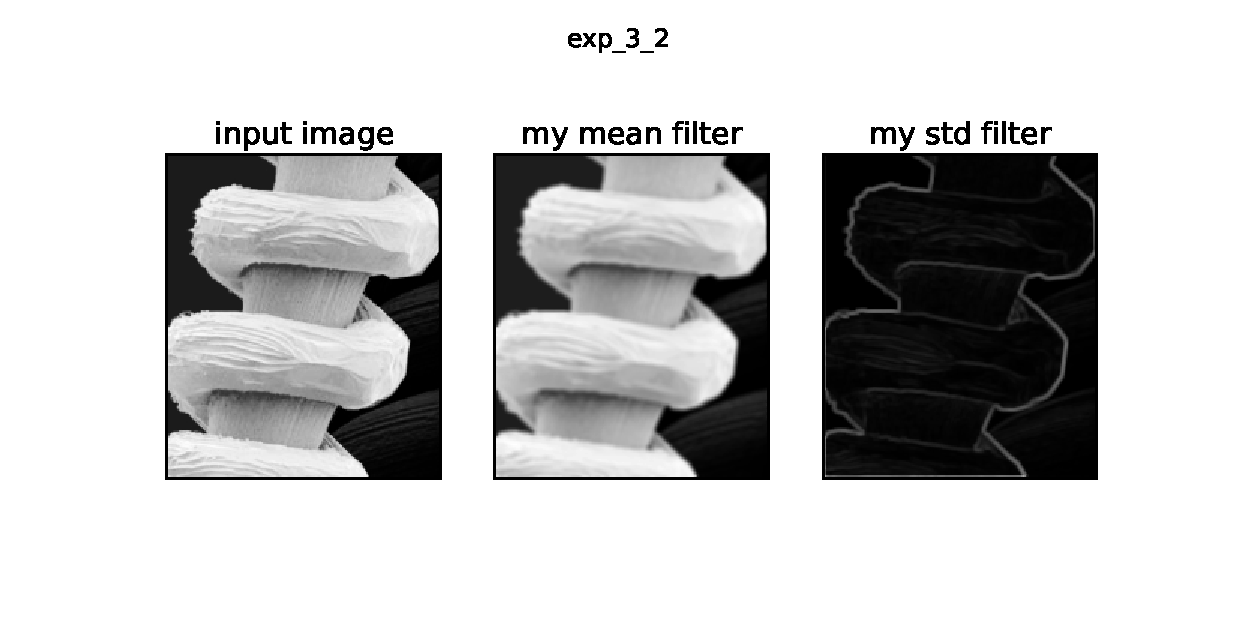
\includegraphics[width=30pc]{exp_3_2.eps}
	\caption{(a)步骤2实验结果}
\end{figure}
\subsubsection{步骤3}
我是用正态分布函数来模拟高斯白噪声的函数,然后用的$5\times5$的邻域平均。从实验结果上看$5\times5$的效果不是特别好。邻域平均做为一种积分运算,会导致图像模糊是肯定的,但其对于噪声的去除性能也不是太好,我觉得出于防止模糊的角度除法,窗口模板不能取得太大,但是窗口模板小取平均值并不能逼近其期望值。
\begin{figure}[h]
	\centering
	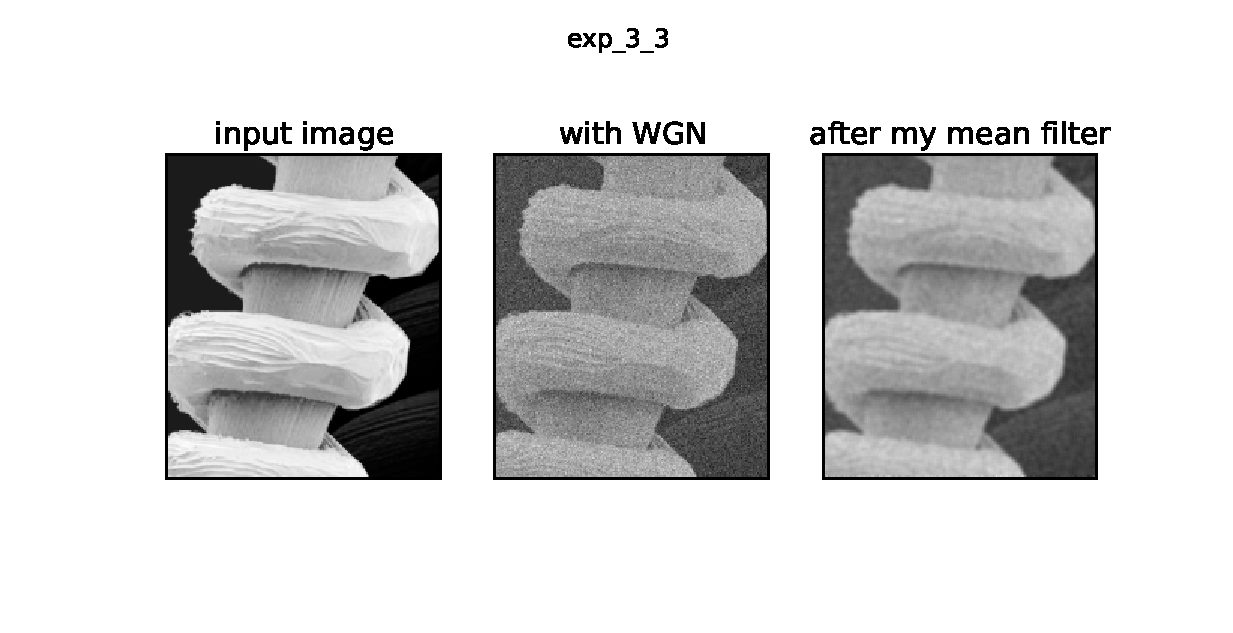
\includegraphics[width=30pc]{exp_3_3.eps}\\
	\caption{(b)步骤3实验结果}
\end{figure}
就像本图所示的一样,均值滤波这种方法挺平庸的。
\subsubsection{步骤4}
由于我只能按照定义写出一个均值滤波的函数,故而难以对比。matlab下有两个函数对二维图像进行处理,matlab是闭源的,我也不知道怎么看出这两个实现有什么区别。水木上有人说除了一些核心库函数,大部分的函数还是可以type出来的,但我还没搞懂怎么做。于是我就用matlab运行了以下,filter2只需要0.004秒,而nlfilter需要3.463秒,而我自己写的均值滤波函数为2.88秒。结果如所示。
\begin{figure}[h]
	\centering
	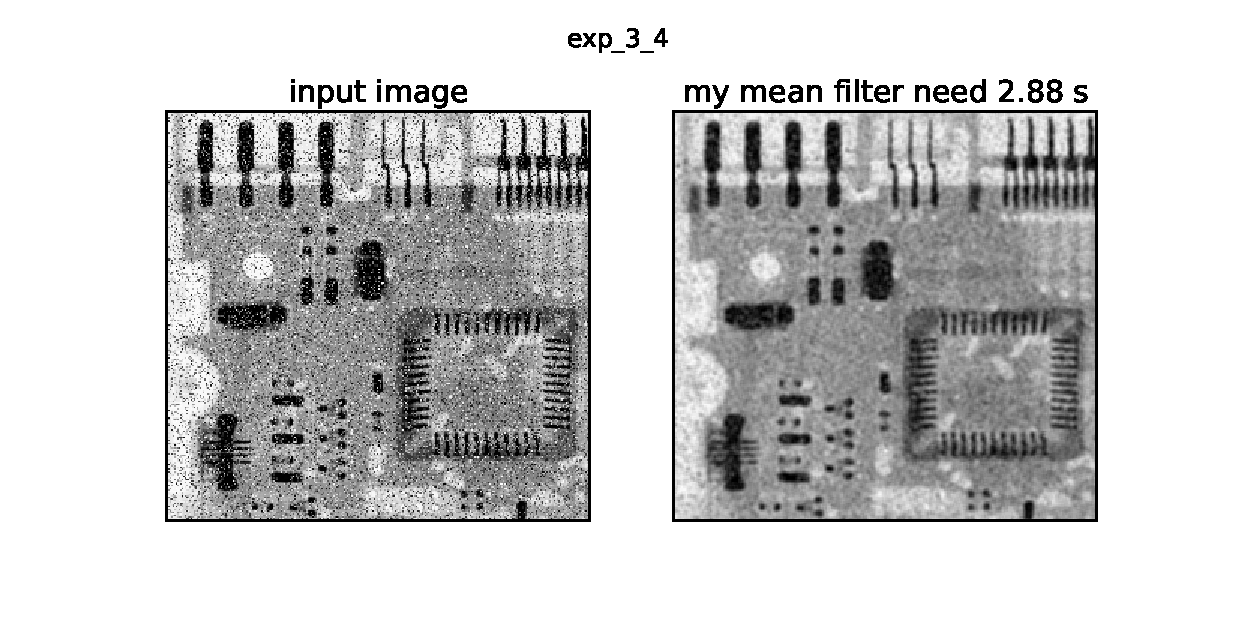
\includegraphics[width=30pc]{exp_3_4.eps}
	\caption{(c)  matlab's filter2 need 0.004 s, matlab's nlfilter need 3.463 s}
\end{figure}
Matlab语言和Python语言一样都是解释型语言,速度至少比属于编译型语言的C/C++慢上一个数量级以上。我自己写的中值滤波是用Python写的,时间与nlfilter差不多,比filter2满好几个数量级,可以猜出nlfilter使用matlab语言写的,filter2是调用的C语言或者Fortran。
可见纯Python的速度还比Matlab快上一点,如果等到PyPy完善后,如果Matlab不是靠它那些强大的toolbox,简直可以直接秒杀之。现在CS搞神经网络等的已经很有往Python转的趋势了,当然EE也许会转向刚出来的Julia,毕竟语法跟Matlab很像,速度又接近C++。
\subsubsection{步骤5}
这一步骤我用的是scipy里自带medfilt2d函数,numpy,scipy这些类库底层都是用C或者fortran写的,速度肯定快,耗时0.040秒。实验原图里的噪声是黑点白点分布,是典型的椒盐噪声,而中值滤波对于椒盐噪声有很好的处理效果,下图就是恢复后的图像,可见恢复后的图像还是很清晰的。
\begin{figure}[h]
	\centering
	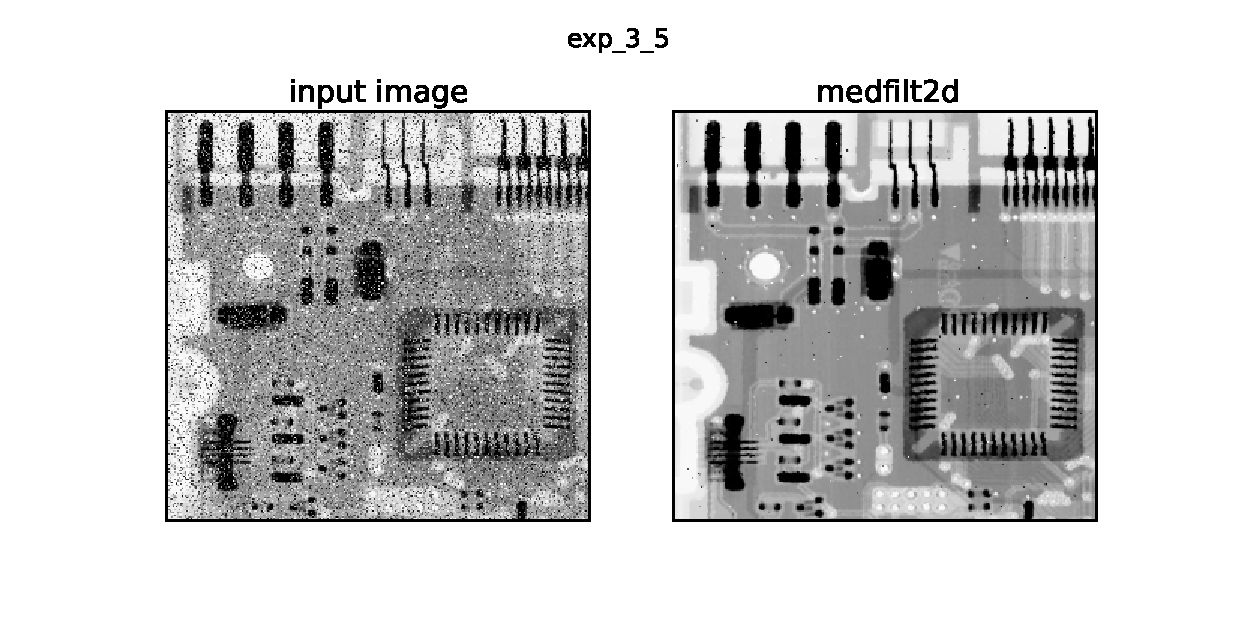
\includegraphics[width=25pc]{exp_3_5.eps}
	\caption{(d)步骤5实验结果}
\end{figure}
\subsubsection{步骤6}
该步骤使用自己编写的中值滤波函数,跟上一步骤medfilt2d的函数的结果相比,肉眼并看不出区别,但是由于我用的python,速度慢上很多,需要5.540秒,跟上一步骤的0.040秒比起来,更加期待Julia和PyPy了。
\begin{figure}
	\centering
	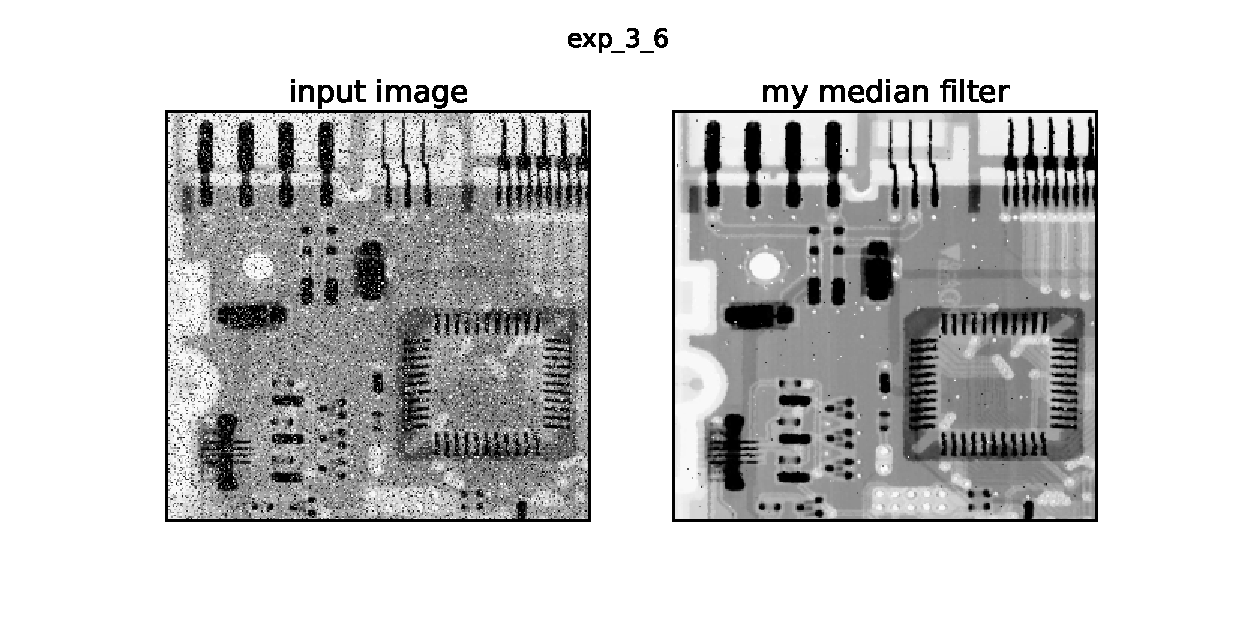
\includegraphics[width=30pc]{exp_3_6.eps}
	\caption{(e)步骤6实验结果}
\end{figure}
\section{心得体会}
在本次实验除了加深了对中值滤波和均值滤波的理解外,我还体会到了算法的优劣和语言类型的选取的重要性,这两个因素都是决定运行时间或者说性能的至关重要的,我觉得我有必要对于Python之外的语言如Julia和C,PyPy都要有一定了解,这样才能在以后的学习工作中选取对自己开发最有力的工具。
\section{实验程序}
随实验报告的文件夹内有Python和Matlab的源程序,由于这是PyEE的一部分,最新的程序会放在github的PyEE项目上。本实验中涉及的函数在PyDSP项目内。
\end{document}
